% O capitulo 4 deve tratar da implementação em si e do resultado.

% Primeiro fazer uma breve introdução ao que será abordado no capitulo e os problemas mais gerais a ser resolvidos.

% Na primeira parte: Descrever a implementação da API de implementação mais interna. Problema: Implementação de uma API coesa que seja capaz de extrair as mensagens de uma conta do WPP. 

    % Escolha da linguagem GO. Escolha da API GO que está sendo usada internamente em detrimento das demais técnicas.
    % Encapsulamento dessa API e apresentação da interface da Api WppScrapper.
    % Exemplo de código encapsulado por essa API.
    % Introduzir exemplo de uso com a implementação da GUI
%
%
% 
% 
% 
% 

\chapter{WppScrapper}
\label{app:name}

Com a intenção cumprir com os objetivos descritos na seção \ref{cap:proposta}, o presente trabalho propõe a criação de uma aplicação onde o usuário poderá configurar uma conta de WhatsApp e realizar a coleta de mensagens. Tal aplicação poderá ser instalada em um computador doméstico simples para ser utilizada pelo usuário e terá uma interface visual gráfica. A essa ferramenta dá-se o nome de \textit{WppScrapperGUI}.

Como parte da proposta também consta a criação de uma API capaz das mesmas tarefas, mas que deve ser implementada de forma agnóstica a como será apresentada para o usuário ou a sua interface de usuário. A essa API dá-se o nome de \textit{WppScrapper}.

No presente capítulo é possível encontrar descrição das decisões técnicas por trás da implementação do \textit{WppScrapper}, tal como sua interface de programação e a utilização da mesma na implementação da \textit{WppScrapperGUI}. Também está presente aqui exemplos de uso da \textit{WppScrapperGUI}.

\section{Implementação da WppScrapper}
\label{cap:wppscrapper}

O primeiro e principal problema a ser revolvido para que a proposta desse trabalho possa ser entregue está na técnica pra extrair as mensagens trocadas através do WhatsApp. Como já mostrado na seção \ref{cap:trabalhosrelacionados}, os trabalhos relacionados procuram resolver esse problema de duas formas. Uma delas é extraindo as mensagens diretamente do dispositivo móvel, acessando o banco de dados e descriptografando-o, e a outra consiste em extraí-las da página do \textit{WhatsApp Web} utilizando de técnicas de \textit{Web Scrapping}.

Para a implementação deste trabalho ficou decido utilizar uma API de terceiro que provê uma reimplementação da API do WhatsApp Web. Essa API, a \textit{GOWhatsApp}\footnote{https://github.com/Rhymen/go-whatsapp}, consiste na implementação da engenharia reversa da API do WhatsApp Web de forma que tal implementação é capaz de se comunicar diretamente com o servidor do WhatsApp Web e prover uma interface de programação igual, ou próxima, à interface \textit{WebSocket} usada internamente pelo WhatsApp Web.

O uso da \textit{GOWhatsApp} é justificado pela facilidade que a mesma provê para que se possa obter os dados que a aplicação aqui proposta necessita. Mas, apesar de mais fácil, ainda se fez necessário encapsular essa API e prover uma outra que seja mais direta ao suprir os objetivos do trabalho atual, como extrair as mensagens para um arquivo \textit{CSV}. Além disso, esse encapsulamento também se justifica pela necessidade de que a API \textit{WppScrapper} não dependa demais dessa API de terceiro e que a forma de obtenção dos dados possa ser trocada sem que a interface mude. Ou seja, os programas que utilizarem a \textit{WppScrapper} não precisarão mudar sua implementação caso o \textit{WppScrapper} mude a forma de acessar os dados internamente; assim, o \textit{GO WhatsApp} poderá ser substituído futuramente sem impactar a interface gráfica, que será apresentada mais adiante, e nem nenhum outro programa que possa surgir futuramente.

A API \textit{GO WhatsApp} é escrita usando a linguagem de programação \textit{GO}\footnote{https://golang.org/}. Esse fato não torna mandatório que o resto do projeto aqui desenvolvido seja feito usando essa mesma linguagem, pois existem ferramentas da linguagem que possibilitam que suas funções sejam executadas de outras linguagens. Mas ficou decidido implementar a API WppScrapper também nesta linguagem devido às facilidades e suas características. 

O presente trabalho objetiva implementar também um programa com interface gráfica de usuário que utiliza a API que está sendo descrita no presente capítulo e apresenta ao usuário suas funções. A linguagem GO permitirá que esse programa possa ser executado em qualquer sistema operacional com facilidade, pois ao realizar a exportação do executável, o compilador da linguagem embute todas as dependências e tem como resultado um único arquivo. Esse compilador é construído para conseguir exportar para todos os principais sistemas operacionais modernos e seus programas serem executados sem a necessidade de instalação ou configuração de nenhuma dependência adicional. Esse objetivo é herdado da linguagem para as demais ferramentas e APIs construídas usando-a. Dessa forma, mesmo que haja a necessidade do uso de um \textit{framework} ou uma biblioteca específica, dificilmente a mesma limitará as plataformas que será possível executar o programa final ou adicionará necessidades que dificultem sua instalação e uso.

Além disso, também foi avaliado o fato de ser uma linguagem de código aberto, ter uma comunidade ativa dando suporte não só na manutenção e desenvolvimento da linguagem em si, mas também a uma sorte enorme de APIs e ferramentas feitas com e para a linguagem, uma documentação bem escrita e uma sintaxe limpa e familiar. 

% \begin{figure}[h!]
%     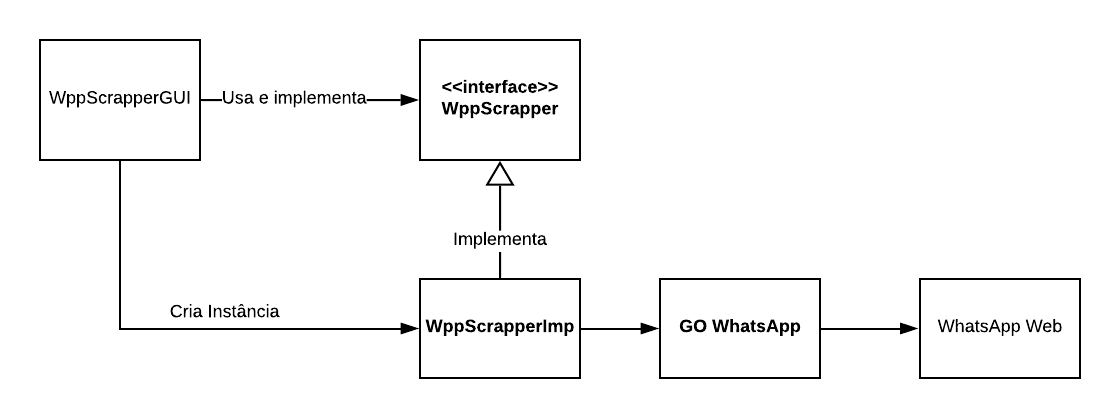
\includegraphics[width=\textwidth]{img/WppScrapperAPIs.png}
%     \caption{Diagrama de pacotes que demonstra como uma aplicação usuária da API \textit{WppScrapper}, exemplificada com o nome de \textit{WppScrapperGUI}, se relaciona com o \textit{WppScrapper} e sua implementação concreta, a \textit{WppScrapperImp}.}
%     \centering
%     \label{fig:WppScrapperAPIs}
% \end{figure}

Como visto anteriormente, a interface da \textit{WppScrapper} precisará ser sólida e agnóstica a detalhes de implementação interna. No diagrama da figura \ref{fig:WppScrapperClass} está ilustrado o que está aqui idealizado: o programa \textit{WppScrapperGUI} precisará referenciar a implementação concreta do \textit{WppScrapper} apenas no momento de criar a instância, diminuindo o impacto de mudanças internas. Tal como o \textit{WppScrapperGUI} o mesmo deve ser verdade para qualquer programa que use a API \textit{WppScrapper} para extrair mensagens trocadas por meio do WhatsApp.

\begin{figure}[!htb]
    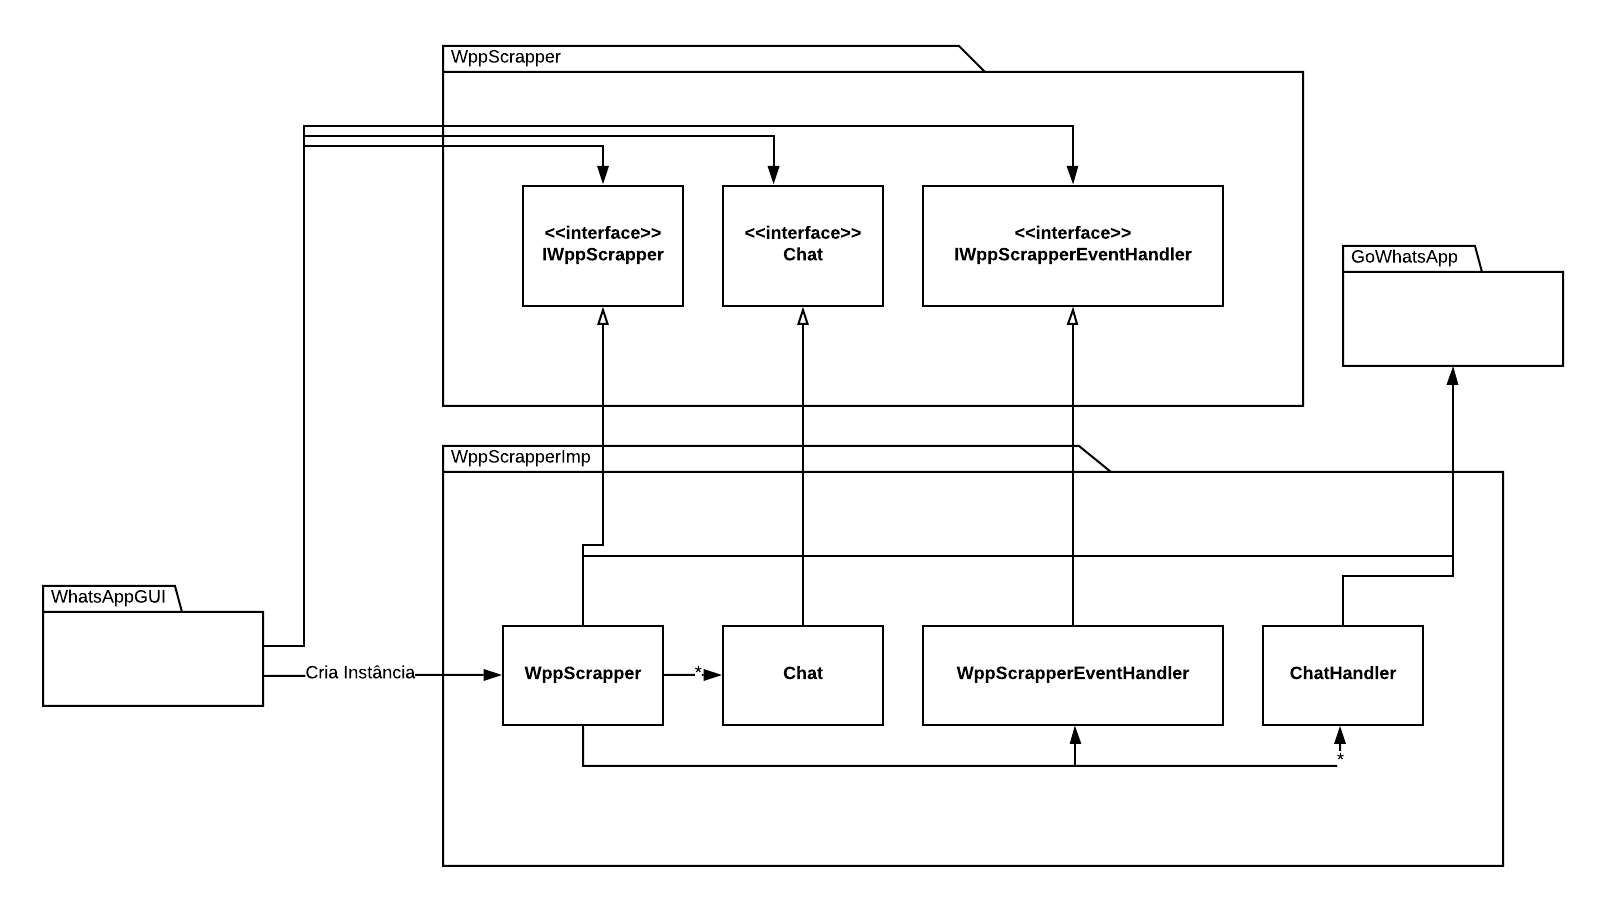
\includegraphics[width=\textwidth]{img/WppScrapperClass.png}
    \caption{Diagrama de pacotes simplificado com diagrama de classes simplificado que demonstra como o \textit{WppScrapper} se relaciona com o \textit{WppScrapperImp}, \textit{WppScrapperGUI} e com a API \textit{GoWhatsApp}.}
    \centering
    \label{fig:WppScrapperClass}
\end{figure}

A figura \ref{fig:WppScrapperInterfaces} descreve um diagrama de classes com a definição das interfaces de programação resultado de todos os requisitos descritos na  seção \ref{cap:proposta}. O usuário da API poderá instanciar uma implementação concreta da interface \textit{IWppScrapper} e através dela ter acesso às funcionalidades desejadas. Esse usuário também poderá implementar as interfaces que possuem sufixo \textit{Listener} e, usando a instância de \textit{IWppScrapperEventHandler} que é provida pela implementação de \textit{IWppScrapper} através da função \textit{GetAppScrapperEventHandler}, adicionar e remover \textit{Listeners} para receber os eventos desejados e poder responder a eles.

% \begin{tikzpicture} 
% \umlclass[type=interface, scale=0.7]{IWppScrapper}{
% }{
%  + Auth(qrChan chan <- string) (string, error) \\
%  + ReAuth(qrChan chan <- string, uuid string) (string, error) \\
%  + WaitInitialization() chan bool \\
%  + Initialized() bool \\
%  + GetChats() map[string]Chat \\
%  + StartScrapper(resume bool) \\
%  + StopScrapper() \\
%  + GetWppScrapperEventHandler() IWppScrapperEventHandler \\
% }
% \umlclass[type=interface, scale=0.7, x=-2,y=-6]{Chat}{
% }{
%  + Name() string \\
%  + Jid() string \\
%  + GetStatus() ChatStatus \\
% }

% \umlclass[type=interface, scale=0.7, x=5.5,y=-8]{IWppScrapperEventHandler}{
% }{
%     + AddOnScrapperStartedListenner(IWppScrapperStartedListener) \\
% 	+ AddOnScrapperStoppedListenner(IWppScrapperStoppedListener)\\
% 	+ AddOnScrapperFinishedListenner(IWppScrapperFinishedListener)\\
% 	+ AddOnChatScrapStartedListenner(IWppScrapperChatScrapStartedListener)\\
% 	+ AddOnChatScrapFinishedListenner(IWppScrapperChatScrapFinishedListener)\\

% 	+ RemoveOnScrapperStartedListenner(IWppScrapperStartedListener)\\
% 	+ RemoveOnScrapperStoppedListenner(IWppScrapperStoppedListener)\\
% 	+ RemoveOnScrapperFinishedListenner(IWppScrapperFinishedListener)\\
% 	+ RemoveOnChatScrapStartedListenner(IWppScrapperChatScrapStartedListener)\\
% 	+ RemoveOnChatScrapFinishedListenner(IWppScrapperChatScrapFinishedListener)\\
% }
% \umlclass[type=interface, scale=0.7, x=-1,y=-13]{IWppScrapperStartedListener}{
% }{
% 	OnWppScrapperStarted(wppScrapper IWppScrapper)

% }
% \umlclass[type=interface, scale=0.7, x=-1,y=-16]{IWppScrapperStoppedListener}{
% }{
% 	OnWppScrapperStopped(wppScrapper IWppScrapper)

% }
% \umlclass[type=interface, scale=0.7, x=-1,y=-19]{IWppScrapperFinishedListener}{
% }{
% 	OnWppScrapperFinished(wppScrapper IWppScrapper)

% }
% \umlclass[type=interface, scale=0.7, x=6,y=-13]{IWppScrapperChatScrapStartedListener}{
% }{
% 	OnWppScrapperChatScrapStarted(chat Chat)

% }
% \umlclass[type=interface, scale=0.7, x=6,y=-16]{IWppScrapperChatScrapFinishedListener}{
% }{
% 	OnWppScrapperChatScrapFinished(chat Chat)

% }
% \umluniassoc{IWppScrapper}{Chat}
% \umluniassoc{IWppScrapper}{IWppScrapperEventHandler}
% \umluniassoc{IWppScrapperEventHandler}{IWppScrapperChatScrapFinishedListener}
% \end{tikzpicture}

É de responsabilidade da implementação concreta implementar o \textit{IWppScrapperEventHandler} e disparar os eventos no momento correto. A implementação do \textit{WppScrapper} também possui a responsabilidade de implementar todas as outras funções de \textit{IWppScrapper} tal como uma função adicional para criar a instância da classe concreta que implementa tal interface. Na figura \ref{fig:WppScrapperClass} é possível identificar como as referências se dão. É possível ver que o módulo que contém as interfaces principais não possuem qualquer referência para fora do módulo e qualquer dependência da API \textit{GO WhatsApp} é isolada dentro da implementação concreta e pode ser substituída sem causar grandes impactos na interface ou nos usuários da API \textit{WppScrapper}.

\begin{figure}[!htb]
    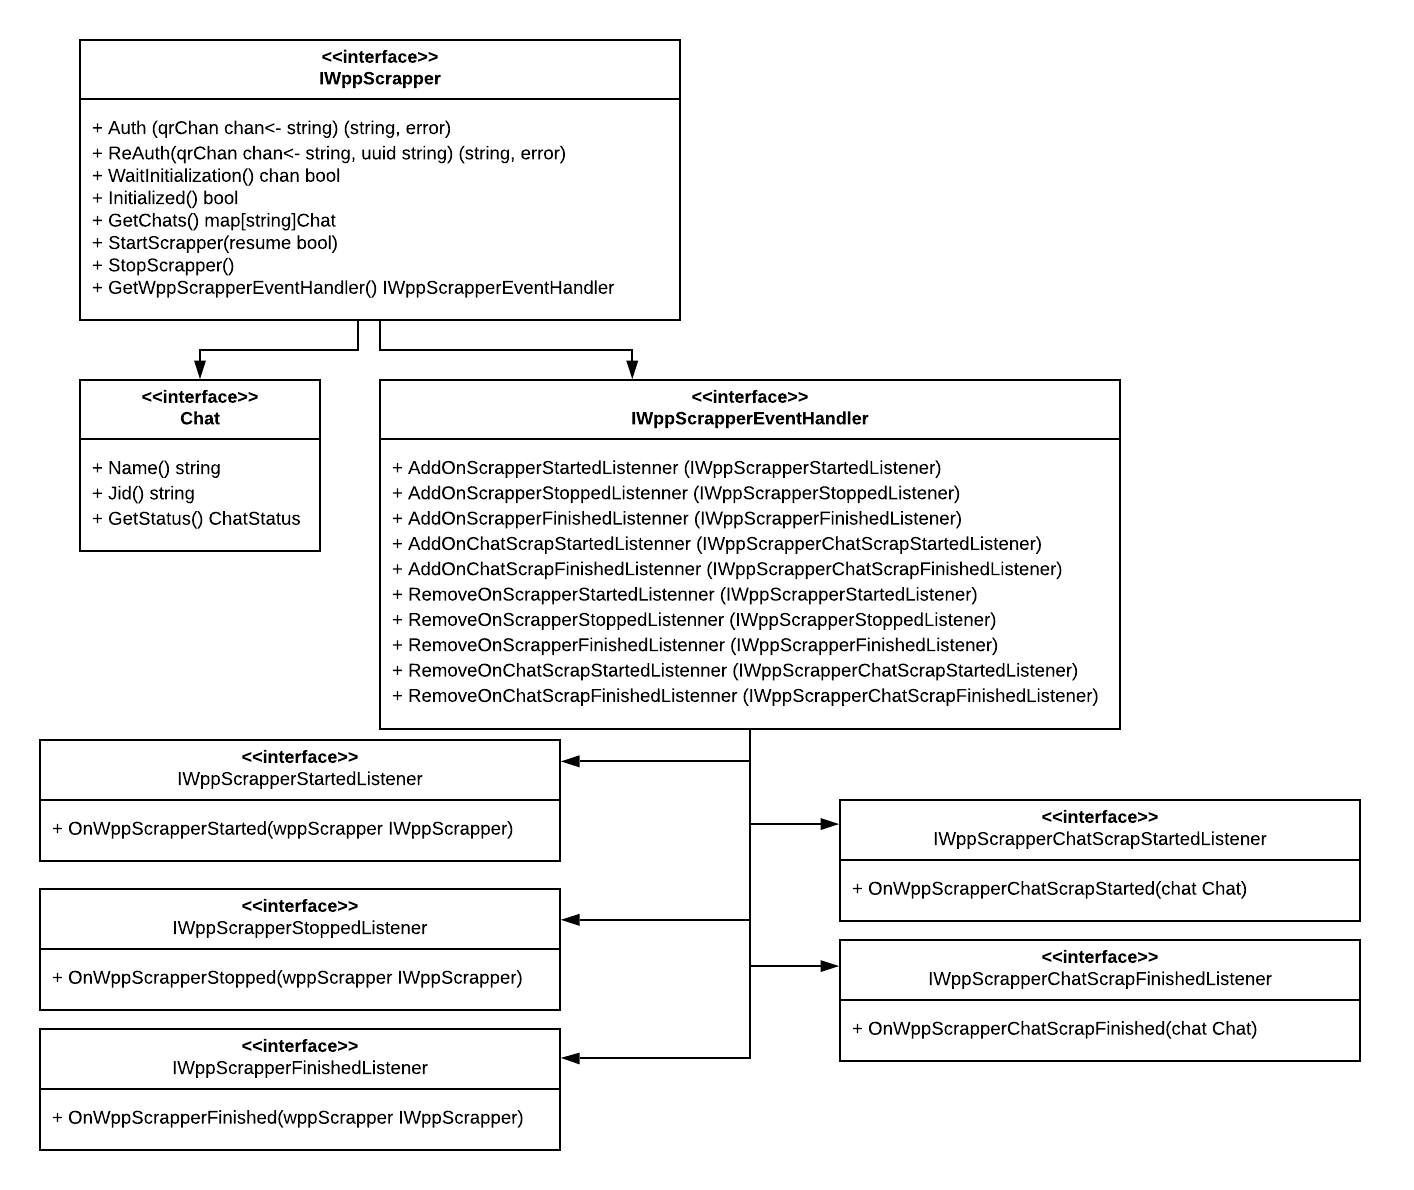
\includegraphics[width=\textwidth]{img/WppScrapperInterface.png}
    \caption{Diagrama de Classes com as interfaces que compõem o \textit{WppScrapper}}
    \centering
    \label{fig:WppScrapperInterfaces}
\end{figure}
Para que haja acesso às informações do WhatsApp, é necessária a autenticação com o uso do \textit{QRCode}. O \textit{WppScrapper} é capaz de recuperar esse \textit{QRCode} através da \textit{GO WhatsApp}. Como é possível ver no diagrama de sequência da figura \ref{fig:UML_Sequence_Auth}, onde está ilustrado o processo de autenticação, o programa recebe de forma assíncrona as informações do \textit{QRCode} e deve passar adiante para o usuário. Uma vez que o usuário realize o escaneamento do \textit{QRCode}, a função é capaz de retornar com sucesso. Não está ilustrado na figura, mas o usuário pode demorar mais que um tempo determinado; caso isso, ocorra a função irá retornar com erro de \textit{timeout}.

\begin{figure}[!htb]
    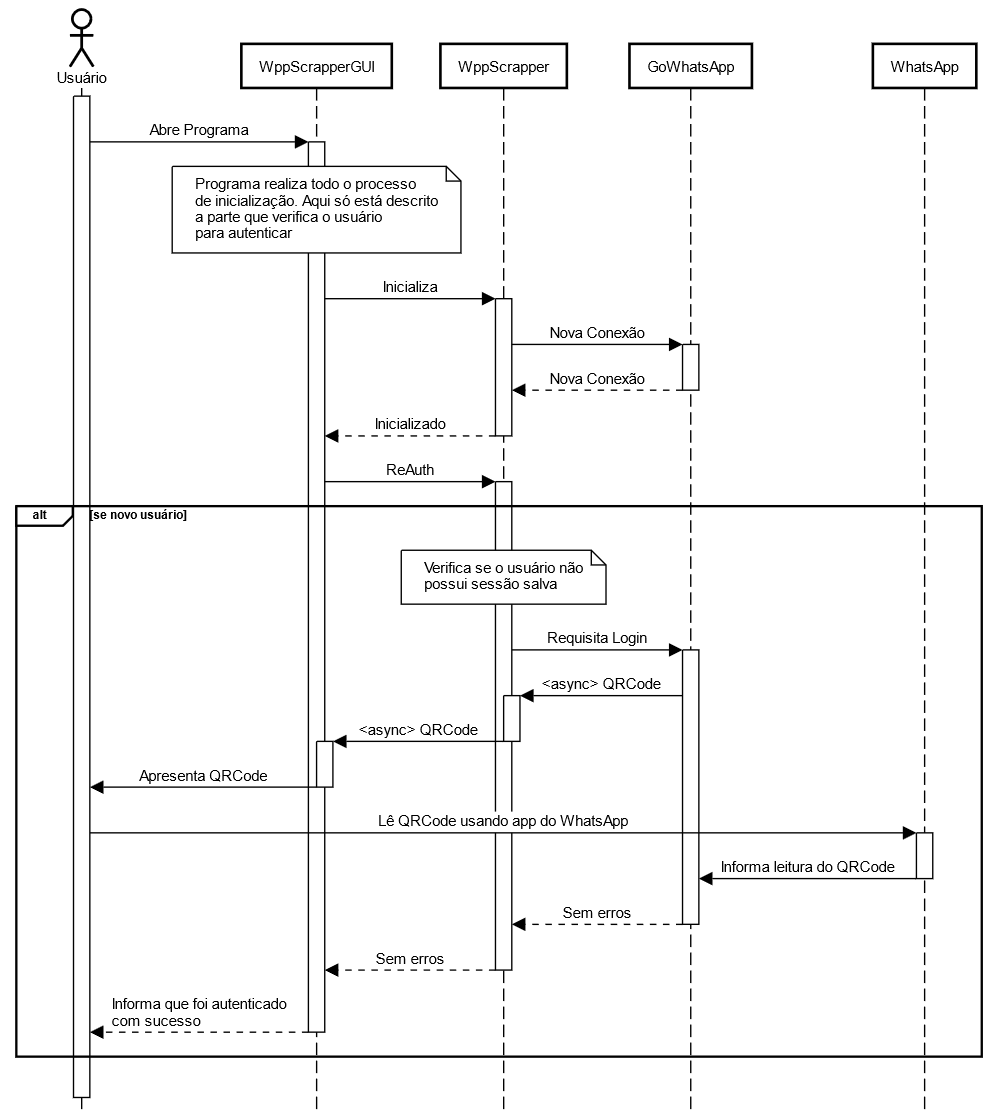
\includegraphics[width=\textwidth]{img/UML_Sequence_Auth.png}
    \caption{Diagrama da sequência que demonstra o processo de autenticação de um usuário sem sessão salva.}
    \centering
    \label{fig:UML_Sequence_Auth}
\end{figure}

Além das funções necessárias para que se requisite a execução de determinadas ações, como a autenticação (\textit{Auth}), inicialização da rotina de extração das mensagens (\textit{StartScrapper}), pausa dessa rotina (\textit{StopScrapper}) etc, o \textit{WppScrapper} também define uma série de eventos necessários para que a aplicação usuária possa responder adequadamente. Por exemplo, para saber quando a extração terminou, a aplicação usuária deverá implementar a interface \textit{IWppScrapperFinishedListerner} e registrar esse objeto junto ao objeto do tipo \textit{IWppScrapperEventHandler} provido pelo \textit{WppScrapper} através da função \textit{GetWppScrapperEventHandler}. Uma vez que esse objeto estiver registrado, ele terá a função \textit{OnWppScrapperFinished} chamada quando a extração foi concluída. A figura \ref{fig:UML_Sequence_EventAndStart} exemplifica esse processo. De maneira análoga, ocorre com os demais eventos, todos descritos no diagrama de classes da figura \ref{fig:WppScrapperInterfaces} com o sufixo \textit{Listener}.

% Para que a \textit{WppScrapperGUI} possa saber quando a extração das mensagens finalizou, ou quando a extração de alguma conversa específica terminou, dentre outros eventos, e poder responder a esses eventos de forma adequada, foi implementado uma série de eventos. Esses eventos podem ser escutados através das interfaces de sufixo Listener ilustradas na figura \ref{fig:WppScrapperInterfaces}. Na figura \ref{fig:UML_Sequence_EventAndStart} está ilustrado um diagrama de sequencia que exemplifica o processo de escutar o evento \textit{OnScrapperFinishedEvent}, que é disparado no momento em que o \textit{WppScrapper} finaliza de extrair todas as mensagens de todas as conversas.

\begin{figure}[h!]
    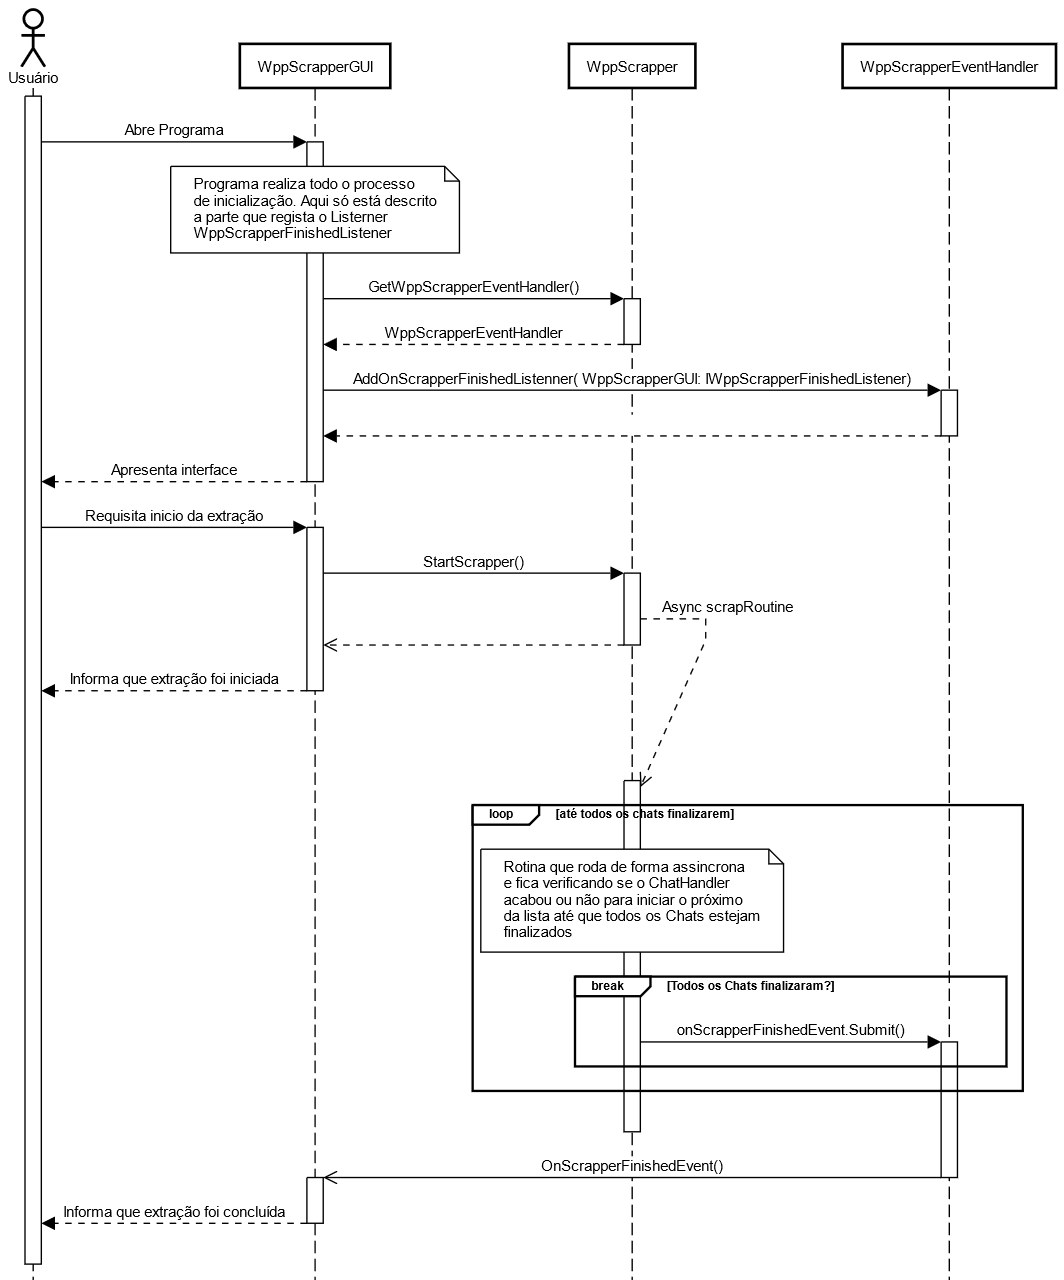
\includegraphics[width=\textwidth]{img/UML_Sequence_EventAndStart.png}
    \caption{Diagrama da sequência que demonstra o processo de registrar o \textit{Listerner} \textit{IWppScrapperFinishedListerner} até o momento que o mesmo é acionado.}
    \centering
    \label{fig:UML_Sequence_EventAndStart}
\end{figure}

Na próxima sessão, estará descrito o processo de implementação da \textit{WppScrapperGUI}. Junto a isso será possível encontrar mais exemplos de uso da \textit{WppScrapper}.

\section{Implementação da WppScrapperGUI}

Para realizar a implementação do \textit{WppScrapperGUI}, o primeiro desafio está na escolha de uma biblioteca de construção interface gráfica escrita na linguagem GO que atenda as necessidades. Ou seja, essa biblioteca deveria permitir que o programa resultante seja executado nos diferentes sistemas operacionais, (\textit{e.g.} \textit{Windows}, \textit{Linux}), que seja estável, tenha uma interface de programação bem documentada e estruturada, possua o conjunto de funcionalidades e elementos visuais e interativos necessários, (\textit{e.g Botão, Texto, Tabela, Imagem}) e que a interface gráfica gerada por ela seja agradável aos olhos do usuário.

Dentre as bibliotecas estudadas e testadas, aquela se mostrou melhor para atender as necessidades do projeto foi a \textit{Fyne.io}\footnote{https://fyne.io/}. A facilidade para gerar os programas executáveis para diferentes plataformas, a simplicidade da biblioteca de construção da interface gráfica, boa documentação, o \textit{design} padrão aceitável da interface gerada e ser de código aberto foram as características que foram decisivas para que tenha sido a escolhida.

Para atender aos requisitos definidos no capítulo \ref{cap:proposta}, a interface de usuário implementa duas telas. A primeira é a tela de autenticação, onde o QRCode é apresentado para o usuário e a segunda tela é onde, uma vez autenticado, o usuário poderá iniciar a extração das mensagens. O \textit{WppScrapperGUI} ainda apresenta uma terceira tela de carregamento. Nela não é possível nenhuma interação e é apresentada enquanto alguma operação de transição entre as telas está sendo realizada.

Na figura \ref{fig:Code_Main_Func} está apresentado o trecho do código responsável pela iniciação do programa. É iniciado como variáveis globais as referências às partes principais da biblioteca do \textit{Fyne.io}, pelas quais será possível alterar o conteúdo da janela visível ao usuário, e com uma referência a uma instância do \textit{IWppScrapper}, que foi explicado no capitulo \ref{cap:wppscrapper}. Na função \textit{main} é configurado o tamanho da janela e então chamado a função \textit{ShowAndRun} do \textit{Fyne.io}, que é quando uma janela é aberta, apresentada ao usuário e toda a biblioteca do \textit{Fyne.io} passa a ser executada.

\begin{figure}[h!]
    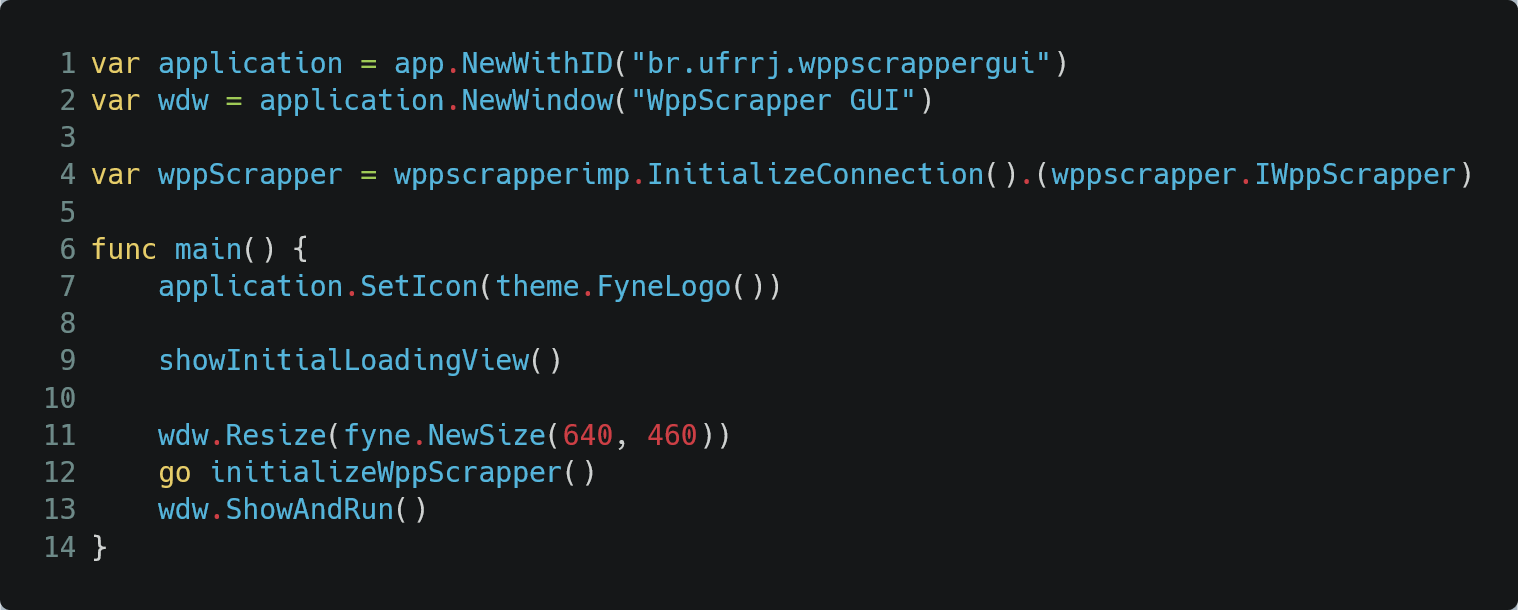
\includegraphics[width=\textwidth]{img/code_main_func.png}
    \caption{Trecho de inicialização do \textit{WppScrapperGUI}.}
    \centering
    \label{fig:Code_Main_Func}
\end{figure}

Ainda na figura \ref{fig:Code_Main_Func} é possível ver que há a chamada da função \textit{showInitialLoadingView}. Essa função somente apresenta na janela um texto informando ao usuário que o programa está carregando. Nesse mesmo trecho de código tem a chamada assíncrona para função \textit{initializeWppScrapper}, que está inteiramente ilustrada na figura \ref{fig:initializeWppScrapper}. Essa função é responsável por requisitar o \textit{QRCode} para o \textit{WppScrapper} e então passá-lo para a função que irá apresentá-lo na janela. Essa função está ilustrada na figura \ref{fig:code_showQrCodeView} e a janela resultado da função na figura \ref{fig:gui_qrCode}. A função ainda trata que, caso ocorra algum erro, ela será chamada novamente de forma recursiva para que um novo \textit{QRCode} seja requisitado apresentado ao usuário. 

Caso não ocorra erros, ou seja, o usuário realize a leitura do \textit{QRCode} corretamente, é apresentado ao usuário a janela de \textit{carregando} novamente enquanto o WppScrapper não termina de inicializar. Uma vez inicializado, o programa chama a função \textit{showMainView}, que é responsável por requisitar a apresentação da segunda tela, a tela onde é possível iniciar a extração das mensagens.

\begin{figure}[h!]
    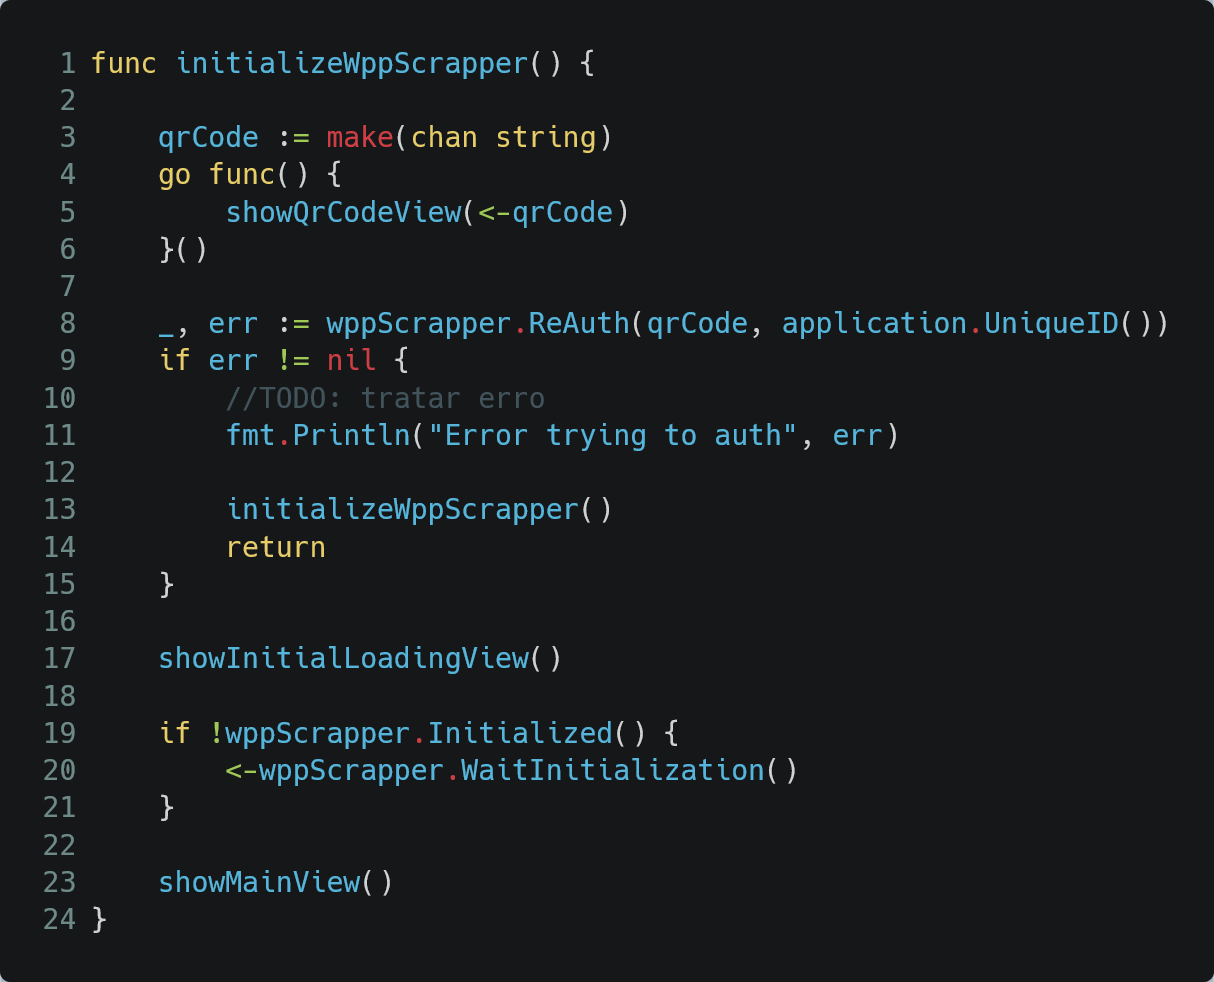
\includegraphics[width=\textwidth]{img/code_initializeWppScrapper.png}
    \caption{Trecho de código que trata a autenticação do usuário.}
    \centering
    \label{fig:initializeWppScrapper}
\end{figure}

\begin{figure}[h!]
    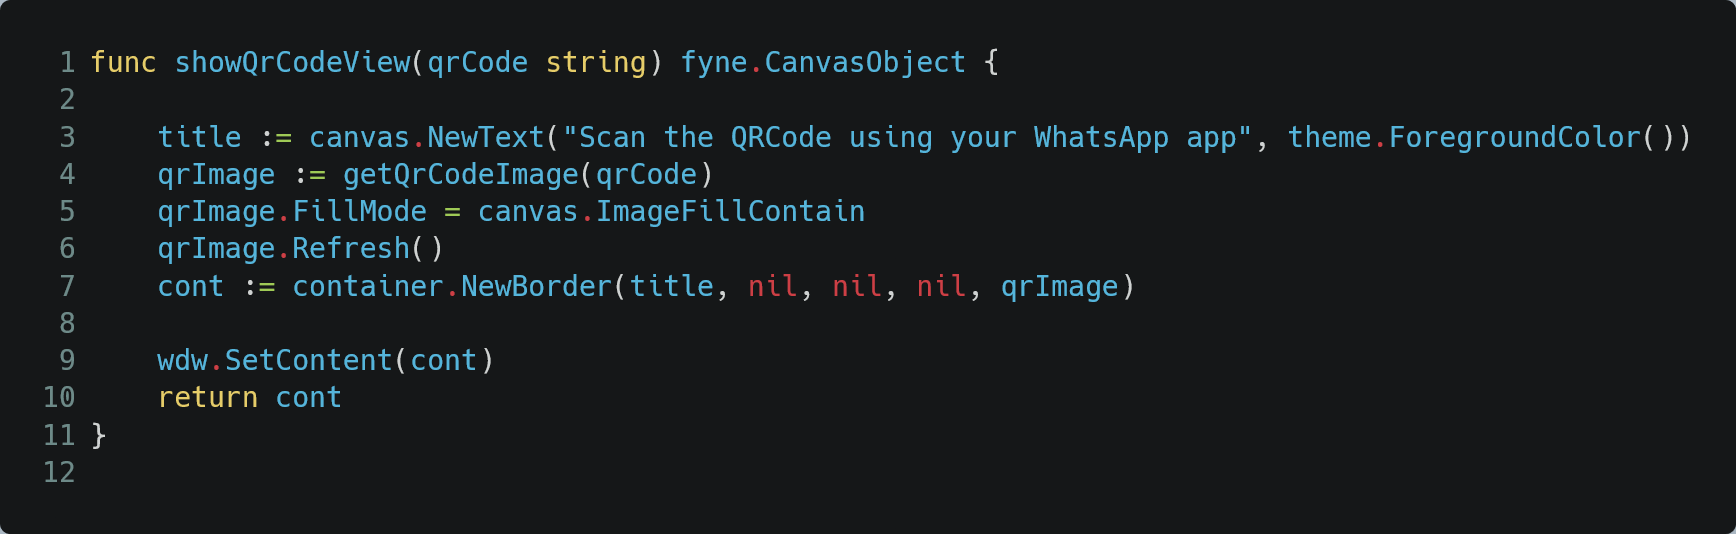
\includegraphics[width=\textwidth]{img/code_showQrCodeView.png}
    \caption{Trecho de código que apresenta o QRCode ao usuário.}
    \centering
    \label{fig:code_showQrCodeView}
\end{figure}

\begin{figure}[h!]
    \centering
    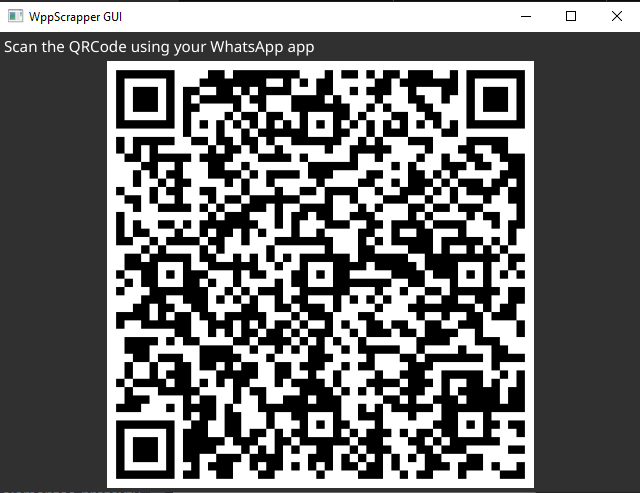
\includegraphics[width=0.5\textwidth]{img/gui_qrCode.png}
    \caption{Janela que apresenta o QRCode ao usuário.}
    \label{fig:gui_qrCode}
\end{figure}

A função \textit{showMainView} apenas cria uma nova instancia do tipo \textit{MainView} e requisita que a mesma apresente seu conteúdo através da função \textit{Show}. Esse tipo é responsável por construir a tela que permite ao usuário iniciar a extração do conteúdo, pausar a mesma e recomeçar, caso deseje. Nessa janela o usuário também tem acesso ao estado atual do programa, \textit{e.g.} executando a extração, esperando, finalizado, tal como informação do estado de cada \textit{Chat}.

Nessa parte do programa é possível encontrar bons exemplos de uso da API \textit{WppScrapper}. Na função \textit{buildHeader}, parcialmente apresentada na figura \ref{fig:code_buildHeader_btns}, é possível ver o código executado quando os botões são acionados pelo usuário. Já na figura \ref{fig:code_listeners} encontramos exemplo de código que implementa os listeners definidos na API \textit{WppScrapper} e usa a mesma API para assinar a instancia e passar a 'escutar' caso algum desses eventos ocorra. Assim o programa pode responder e esconder determinados botões a depender do estado do programa, como por exemplo esconde os botões que iniciam a extração das mensagens quando o programa já está extraindo as mensagens e apresentar apenas o botão que pausa essa execução.

\begin{figure}[h!]
    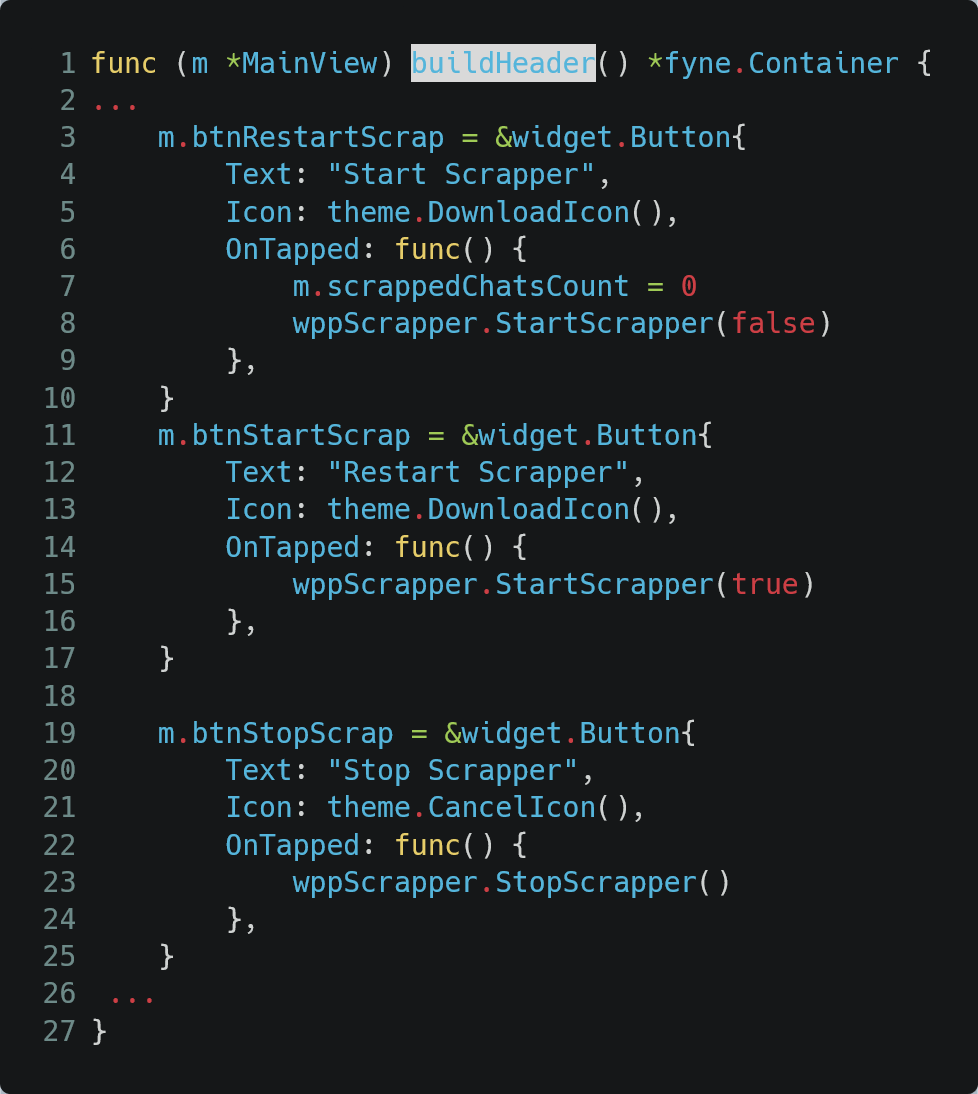
\includegraphics[width=\textwidth]{img/code_buildHeader_btns.png}
    \caption{Parte da função \textit{buildHeader} do tipo \textit{MainView} que cria os botões que inicia a extração, pausa a mesma e reinicia. Parte da função foi omitida.}
    \centering
    \label{fig:code_buildHeader_btns}
\end{figure}

\begin{figure}[h!]
    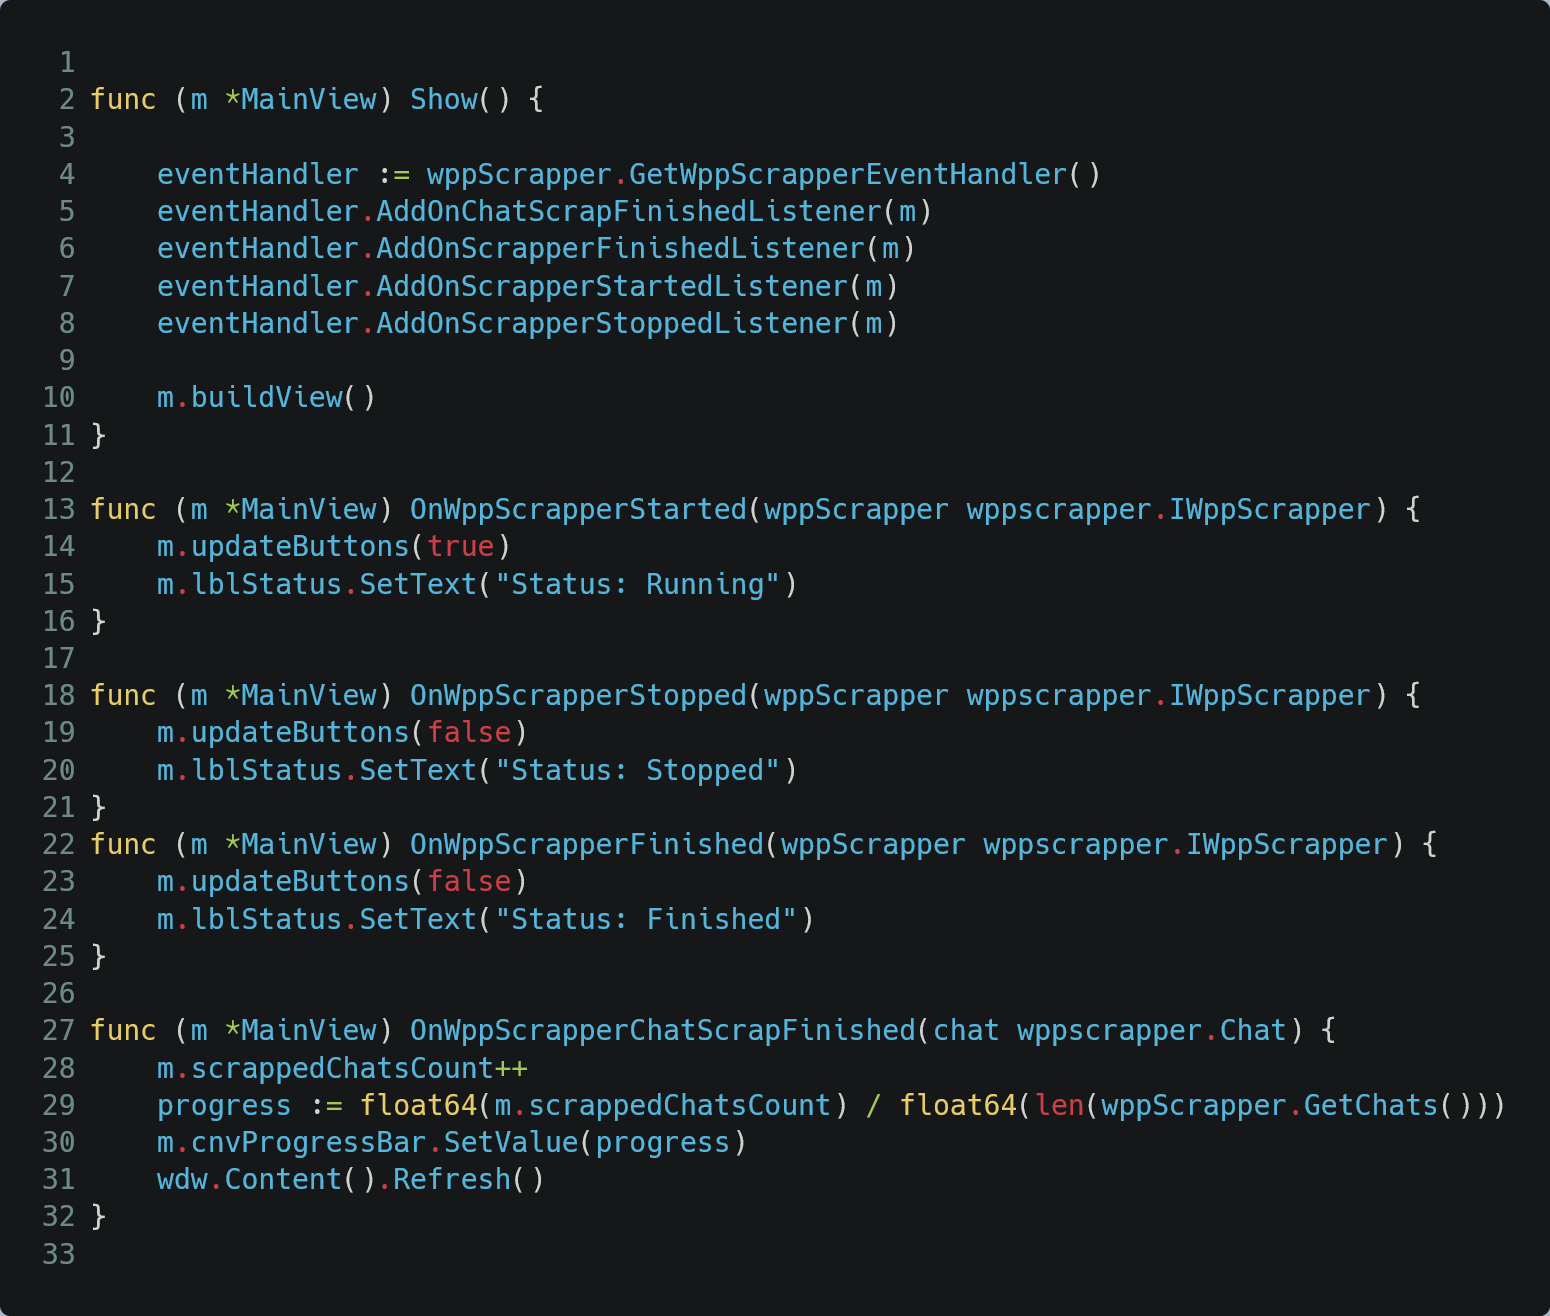
\includegraphics[width=\textwidth]{img/code_listeners.png}
    \caption{Trecho de código que define funções para o tipo \textit{MainView}. Nesse trecho é possível encontrar a implementação das interfaces da API \textit{WppScrapper}.}
    \centering
    \label{fig:code_listeners}
\end{figure}


% Objetivo é implementar uma iterface visual. Não há tantas preocupações arquiteturais pois é um sistema simples onde a logica de negócio ja está implementada no WppScrapper

% Dentre as opções de bibliotecas de interface grafica disponíveis para GO, foi escolhido o Fyne devido a sua facilidade e simplicidade. As possibilidades de customização são limitadas, mas ja ter uma sorte de elementos prontos para uso e de aparencia aceitável é um bom diferencial.

% Alem disso o fyne mantém a possibilidade de realização de build para muiltiplas plataformas do go, disponibilizando uma ferramenta que possibilita contruir aplicação para linux, windows ou osx facilmente de qualquer máquina, bastando essa possuir o go e o docker instalado.

% Uma vez decido a api de interface gráfica, bastava implementar o código que gerava a interface e conectava com o WppScrapper, seja respondendo as mudanças de estado do scrapper quanto realizando chamadas no mesmo.


\section{Demonstração do WppScrapperGUI}

Com intuito de realizar uma pequena demonstração do \textit{WppScrapperGUI} em ação, essa secção descreve um procedimento bastante simplificado de coleta de mensagens de grupos públicos de WhatsApp. Os \textit{links} para acesso aos grupos foram encontrados disponíveis no \textit{Google} e no \textit{Facebook}. Para a realização da operação, foi utilizada uma conta de WhatsApp criada apenas para essa finalidade.

O primeiro passo realizado foi a inscrição dessa conta nos grupos públicos. Como a intenção era realizar apenas uma pequena amostra, foi feita a inscrição em 10 grupos de temas variados, \textit{e.g.} futebol, jogos. As inscrições foram feitas às 20h de um dia e deixou-se coletando as mensagens até às 13h do dia seguinte, quando foi feito o uso do \textit{WppScrapperGUI} para realizar a extração das mensagens. 

Nas figuras \ref{fig:wppscrapper-idle}, \ref{fig:wppscrapper-running2} e \ref{fig:wppscrapper-finished} encontra-se exemplo do programa aberto em seus três diferentes estados. No primeiro o programa acabara de ser aberto e tem listado todas as conversas encontradas em estado de espera, apresentado na figura \ref{fig:wppscrapper-idle}. Em seguida, após acionado pelo usuário a realizar a extração, o programa modifica parte da sua interface para indicar seu estado, apresentar as opções de ação possível e indicar a conversa que está sendo extraído no momento, tal como seu indicador de progresso passa a indicar uma porcentagem referente a quantidade de conversas extraídas frente ao total de conversas a se extrair, ilustrado na figura \ref{fig:wppscrapper-running2}. Por ultimo o programa apresenta a tela de finalizado, onde todas as conversas já foram extraídas e se encontram em formato CSV no computador do usuário na mesma pasta em que se encontra o executável do programa, ilustrado na figura \ref{fig:wppscrapper-finished}.

\begin{figure}[!htb]
    \centering
    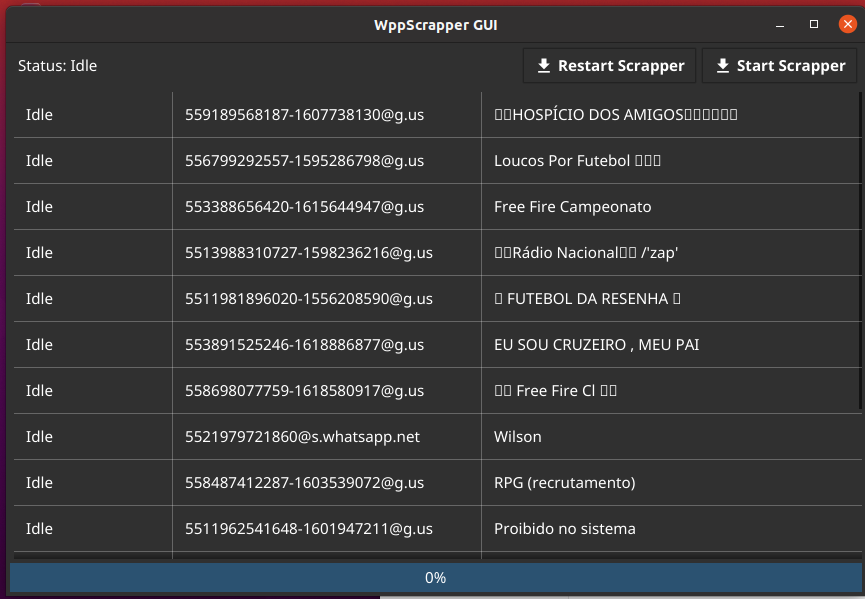
\includegraphics[width=0.8\textwidth]{img/wppscrapper-idle.png}
    \caption{Captura de tela do \textit{WppScrapperGUI} em estado de espera logo após de ter o usuário validado e carregar todas as informações.}
    \label{fig:wppscrapper-idle}
\end{figure}

\begin{figure}[!htb]
    \centering
    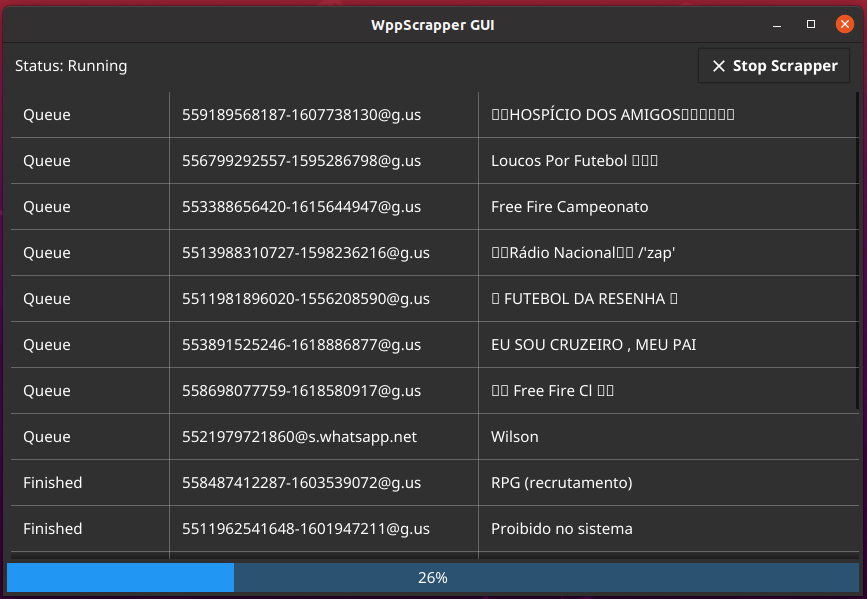
\includegraphics[width=0.8\textwidth]{img/wppscrapper-running2.png}
    \caption{Captura de tela do \textit{WppScrapperGUI} rodando a rotina de extração das mensagens, onde $26\%$ das conversas já foram extraídas.}
    \label{fig:wppscrapper-running2}
\end{figure}

\begin{figure}[!htb]
    \centering
    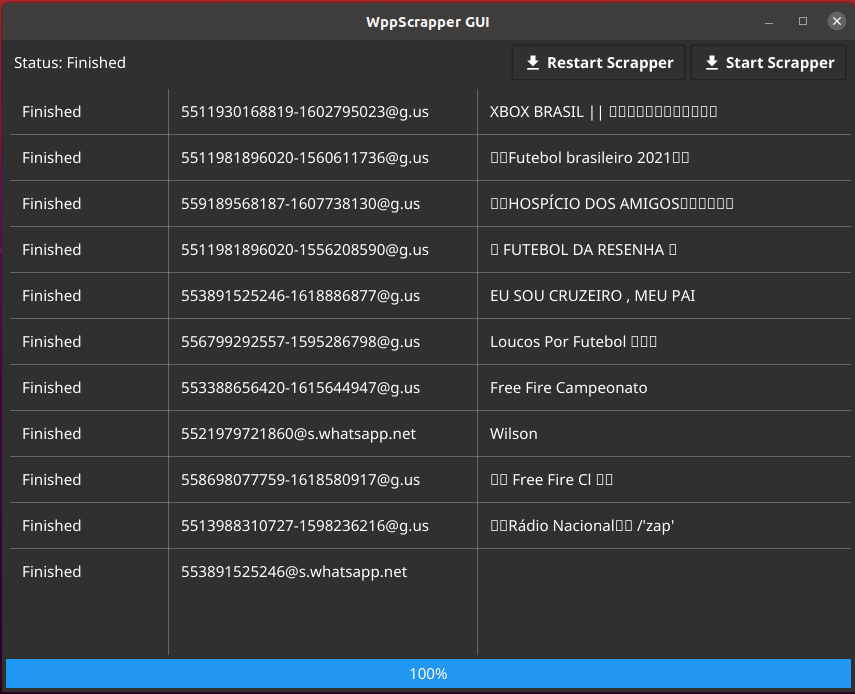
\includegraphics[width=0.8\textwidth]{img/wppscrapper-finished.png}
    \caption{Captura de tela do \textit{WppScrapperGUI} após finalizar de extrair todas as conversas.}
    \label{fig:wppscrapper-finished}
\end{figure}

Neste exemplo, foi possível coletar e extrair um total de 1472 mensagens de 10 diferentes grupos que possuem, no total, 1311 usuários não necessariamente distintos. Na tabela \ref{fig:result} é possível encontrar esses dados descritos para cada grupo tal como seu nome.

% \begin{figure}[!htb]
%     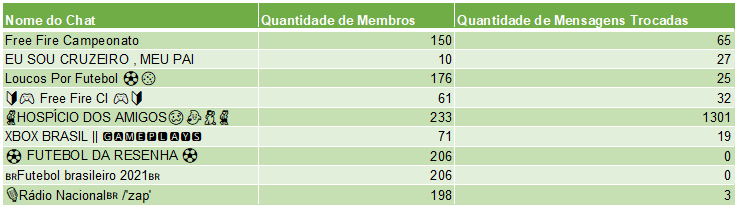
\includegraphics[width=\textwidth]{img/result_extract.png}
%     \caption{Trecho de código que define funções para o tipo \textit{MainView}. Nesse trecho é possível encontrar a implementação das interfaces da API \textit{WppScrapper}.}
%     \centering
%     \label{fig:result}
% \end{figure}


\begin{table}[!htb]
  \centering
  \caption{Tabela de nome dos grupos que tiveram mensagens extraídas com a quantidade de membros e a quantidade de mensagens extraídas por grupo.}
    \label{fig:result}
%   \rowcolors{1}{light-gray}
  \begin{tabular}{l c c c}
  \toprule
    Nome do Chat & Quantidade de Membros & Quantidade de Mensagens \\
    \midrule
        Free Fire Campeonato & 150 & 65  \\
        
        EU SOU CRUZEIRO , MEU PAI & 10 & 27  \\
        
        Loucos Por Futebol & 176 & 25  \\
        
        Free Fire Cl & 61 & 32  \\
        
        HOSPÍCIO DOS AMIGOS & 233 & 1301  \\
        
        XBOX BRASIL & 71 & 19  \\
        
        FUTEBOL DA RESENHA & 206 & 0  \\
        
        Futebol brasileiro 2021 & 206 & 0  \\
        
        Rádio Nacional & 198 & 3  \\
    \bottomrule
  \end{tabular}
\end{table}

A seguir temos exemplos de arquivos extraídos, em todas as imagens os identificadores, que possuem o número de celular em sua composição, foram borrados para preservar privacidade daqueles que enviaram as mensagens e que participam do grupo em questão. Na figura \ref{fig:csv-msgs} é possível observar, entre outras informações, as mensagens enviadas no grupo "Free Fire Campeonato". Com dados do mesmo grupo, na figura \ref{fig:csv-group} está ilustrado as informações do grupo em si, como o identificador do seu criador e a descrição do grupo. O arquivo com os membros deste grupo está ilustrado na imagem \ref{fig:csv-msgs}. 

\begin{figure}[!htb]
    \centering
    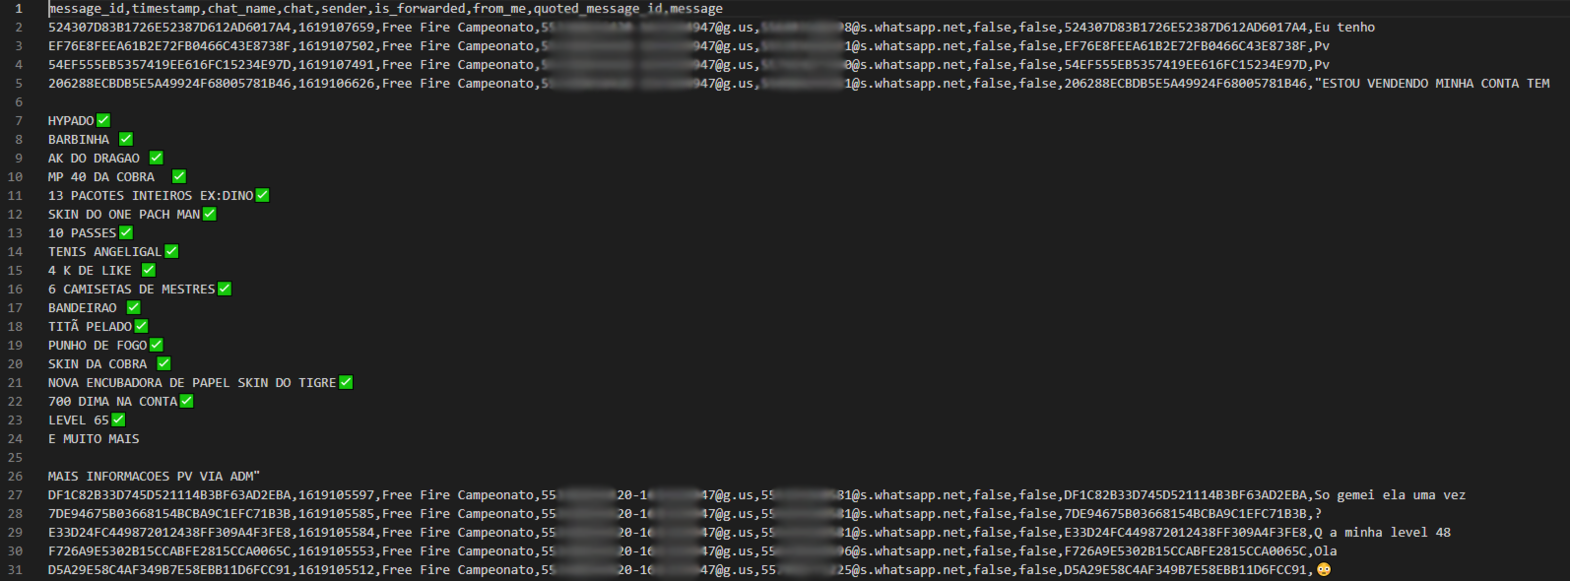
\includegraphics[width=1\textwidth]{img/csv_msgs.png}
    \caption{Captura de tela da parte inicial do conteúdo de um arquivo CSV de mensagens gerado pela extração.}
    \label{fig:csv-msgs}
\end{figure}

\begin{figure}[!htb]
    \centering
    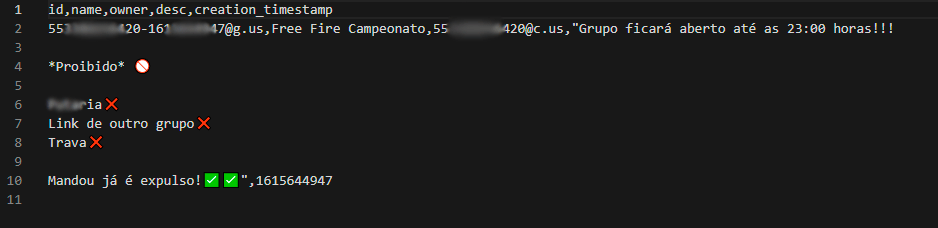
\includegraphics[width=1\textwidth]{img/csv_group.png}
    \caption{Captura de tela do conteúdo um arquivo \textit{CSV} de descrição de um grupo gerado pela extração.}
    \label{fig:csv-group}
\end{figure}

\begin{figure}[!htb]
    \centering
    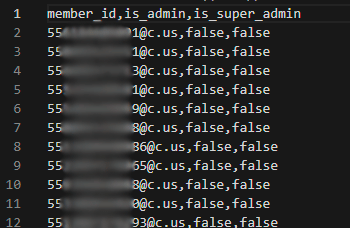
\includegraphics[width=0.7\textwidth]{img/csv_members.png}
    \caption{Captura de tela da parte inicial do conteúdo um arquivo \textit{CSV} de lista de membros de um grupo gerado pela extração.}
    \label{fig:csv-members}
\end{figure}


% \begin{table}[!htb]
% \centering
% \caption{Lista dos parâmetros e seus respectivos valores para cada modelo que será otimizado através do algoritmo genético.}
% \begin{tabular}{llc}
% \toprule
% Modelo                       & Parâmetro                 & Valores \\
% \midrule
% \multirow{6}{*}{Rede Neural} & Variáveis Latentes        & $\{x \mid x = 10 + 10 \cdot i  , 0 \leq  i \leq 9 \} \cup \{150\}$ \\ %[10:10:100..., 150]
%                              & Neurônios                 & $\{x \mid x = 100 + 50 \cdot i  , 0 \leq  i \leq 8 \}$ \\ %[100:50:500...]
%                              & Dropout                   & $\{x \mid x = 0.1 \cdot i  , 0 \leq  i \leq 10 \}$ \\ %[0:0.1:1...]
%                              & Batch                     & $\{64, 128, 256\}$ \\ % [64, 128, 256]
%                              & Épocas                    & $\{10, 20, 30, 50\}$ \\ %[10, 20, 30, 50]
%                              & Paciência                 & $\{1, 2, 3, 4, 5\}$ \\ \midrule %[1, 2, 3, 4, 5]
% IRSVD                        & Variáveis Latentes        & $\{1, 2\} \cup \{x \mid x = 10 \cdot i  , 1 \leq  i \leq 9 \}$ \\ %[1 2 10:10:100...]
%                              & Taxa de Aprendizagem      & $\{x \mid x = 0.01 \cdot i  , 0 \leq  i \leq 10 \}$ \\ % [0:0.01:0.1...]
%                              & Regularização             & $\{x \mid x = 0.01 \cdot i  , 0 \leq  i \leq 10 \}$ \\ \midrule %[0:0.01:0.1...]
% KNN                          & Número Mínimo de Vizinhos & $\{5, 10\}$  \\ %[5 10]
%                              & Número de Vizinhos        & $\{15, 30, 50\}$ \\ %[15 30 50]
% \bottomrule
% \end{tabular}
% \label{tab:gaparam}
% \end{table}